\documentclass[twoside]{book}

% Packages required by doxygen
\usepackage{fixltx2e}
\usepackage{calc}
\usepackage{doxygen}
\usepackage[export]{adjustbox} % also loads graphicx
\usepackage{graphicx}
\usepackage[utf8]{inputenc}
\usepackage{makeidx}
\usepackage{multicol}
\usepackage{multirow}
\PassOptionsToPackage{warn}{textcomp}
\usepackage{textcomp}
\usepackage[nointegrals]{wasysym}
\usepackage[table]{xcolor}

% NLS support packages
\usepackage[ngerman]{babel}

% Font selection
\usepackage[T1]{fontenc}
\usepackage[scaled=.90]{helvet}
\usepackage{courier}
\usepackage{amssymb}
\usepackage{sectsty}
\renewcommand{\familydefault}{\sfdefault}
\allsectionsfont{%
  \fontseries{bc}\selectfont%
  \color{darkgray}%
}
\renewcommand{\DoxyLabelFont}{%
  \fontseries{bc}\selectfont%
  \color{darkgray}%
}
\newcommand{\+}{\discretionary{\mbox{\scriptsize$\hookleftarrow$}}{}{}}

% Page & text layout
\usepackage{geometry}
\geometry{%
  a4paper,%
  top=2.5cm,%
  bottom=2.5cm,%
  left=2.5cm,%
  right=2.5cm%
}
\tolerance=750
\hfuzz=15pt
\hbadness=750
\setlength{\emergencystretch}{15pt}
\setlength{\parindent}{0cm}
\setlength{\parskip}{3ex plus 2ex minus 2ex}
\makeatletter
\renewcommand{\paragraph}{%
  \@startsection{paragraph}{4}{0ex}{-1.0ex}{1.0ex}{%
    \normalfont\normalsize\bfseries\SS@parafont%
  }%
}
\renewcommand{\subparagraph}{%
  \@startsection{subparagraph}{5}{0ex}{-1.0ex}{1.0ex}{%
    \normalfont\normalsize\bfseries\SS@subparafont%
  }%
}
\makeatother

% Headers & footers
\usepackage{fancyhdr}
\pagestyle{fancyplain}
\fancyhead[LE]{\fancyplain{}{\bfseries\thepage}}
\fancyhead[CE]{\fancyplain{}{}}
\fancyhead[RE]{\fancyplain{}{\bfseries\leftmark}}
\fancyhead[LO]{\fancyplain{}{\bfseries\rightmark}}
\fancyhead[CO]{\fancyplain{}{}}
\fancyhead[RO]{\fancyplain{}{\bfseries\thepage}}
\fancyfoot[LE]{\fancyplain{}{}}
\fancyfoot[CE]{\fancyplain{}{}}
\fancyfoot[RE]{\fancyplain{}{\bfseries\scriptsize Erzeugt von Doxygen }}
\fancyfoot[LO]{\fancyplain{}{\bfseries\scriptsize Erzeugt von Doxygen }}
\fancyfoot[CO]{\fancyplain{}{}}
\fancyfoot[RO]{\fancyplain{}{}}
\renewcommand{\footrulewidth}{0.4pt}
\renewcommand{\chaptermark}[1]{%
  \markboth{#1}{}%
}
\renewcommand{\sectionmark}[1]{%
  \markright{\thesection\ #1}%
}

% Indices & bibliography
\usepackage{natbib}
\usepackage[titles]{tocloft}
\setcounter{tocdepth}{3}
\setcounter{secnumdepth}{5}
\makeindex

% Hyperlinks (required, but should be loaded last)
\usepackage{ifpdf}
\ifpdf
  \usepackage[pdftex,pagebackref=true]{hyperref}
\else
  \usepackage[ps2pdf,pagebackref=true]{hyperref}
\fi
\hypersetup{%
  colorlinks=true,%
  linkcolor=blue,%
  citecolor=blue,%
  unicode%
}

% Custom commands
\newcommand{\clearemptydoublepage}{%
  \newpage{\pagestyle{empty}\cleardoublepage}%
}

\usepackage{caption}
\captionsetup{labelsep=space,justification=centering,font={bf},singlelinecheck=off,skip=4pt,position=top}

%===== C O N T E N T S =====

\begin{document}

% Titlepage & ToC
\hypersetup{pageanchor=false,
             bookmarksnumbered=true,
             pdfencoding=unicode
            }
\pagenumbering{alph}
\begin{titlepage}
\vspace*{7cm}
\begin{center}%
{\Large Übung Objektorientierte Programmierung \\[1ex]\large 1.\+0 }\\
\vspace*{1cm}
{\large Erzeugt von Doxygen 1.8.13}\\
\end{center}
\end{titlepage}
\clearemptydoublepage
\pagenumbering{roman}
\tableofcontents
\clearemptydoublepage
\pagenumbering{arabic}
\hypersetup{pageanchor=true}

%--- Begin generated contents ---
\chapter{Hierarchie-\/\+Verzeichnis}
\section{Klassenhierarchie}
Die Liste der Ableitungen ist -\/mit Einschränkungen-\/ alphabetisch sortiert\+:\begin{DoxyCompactList}
\item \contentsline{section}{C\+Counter}{\pageref{class_c_counter}}{}
\begin{DoxyCompactList}
\item \contentsline{section}{C\+Forward\+Counter}{\pageref{class_c_forward_counter}}{}
\item \contentsline{section}{C\+Variable\+Counter}{\pageref{class_c_variable_counter}}{}
\end{DoxyCompactList}
\end{DoxyCompactList}

\chapter{Klassen-\/\+Verzeichnis}
\section{Auflistung der Klassen}
Hier folgt die Aufzählung aller Klassen, Strukturen, Varianten und Schnittstellen mit einer Kurzbeschreibung\+:\begin{DoxyCompactList}
\item\contentsline{section}{\hyperlink{class_c_counter}{C\+Counter} }{\pageref{class_c_counter}}{}
\item\contentsline{section}{\hyperlink{class_c_forward_counter}{C\+Forward\+Counter} }{\pageref{class_c_forward_counter}}{}
\item\contentsline{section}{\hyperlink{class_c_variable_counter}{C\+Variable\+Counter} }{\pageref{class_c_variable_counter}}{}
\end{DoxyCompactList}

\chapter{Datei-\/\+Verzeichnis}
\section{Auflistung der Dateien}
Hier folgt die Aufzählung aller Dateien mit einer Kurzbeschreibung\+:\begin{DoxyCompactList}
\item\contentsline{section}{C\+:/portable\+Dev\+Env\+\_\+2017/workspace2017/project/src/\hyperlink{_c_array_8hpp}{C\+Array.\+hpp} \\*Template-\/\+Klasse \hyperlink{class_c_array}{C\+Array} Erzeugt ein Array vom Typ T mit N Elementen }{\pageref{_c_array_8hpp}}{}
\item\contentsline{section}{C\+:/portable\+Dev\+Env\+\_\+2017/workspace2017/project/src/\hyperlink{_c_array_dec_8cpp}{C\+Array\+Dec.\+cpp} \\*Created on\+: 24.\+05.\+2018 Author\+: diamo }{\pageref{_c_array_dec_8cpp}}{}
\item\contentsline{section}{C\+:/portable\+Dev\+Env\+\_\+2017/workspace2017/project/src/\hyperlink{_c_array_dec_8hpp}{C\+Array\+Dec.\+hpp} \\*L\+ZW Decoder, Dictionary implementiert als Array }{\pageref{_c_array_dec_8hpp}}{}
\item\contentsline{section}{C\+:/portable\+Dev\+Env\+\_\+2017/workspace2017/project/src/\hyperlink{_c_array_enc_8cpp}{C\+Array\+Enc.\+cpp} \\*Created on\+: 24.\+05.\+2018 Author\+: diamo }{\pageref{_c_array_enc_8cpp}}{}
\item\contentsline{section}{C\+:/portable\+Dev\+Env\+\_\+2017/workspace2017/project/src/\hyperlink{_c_array_enc_8hpp}{C\+Array\+Enc.\+hpp} \\*L\+ZW Encoder, Dictionary implementiert als Array }{\pageref{_c_array_enc_8hpp}}{}
\item\contentsline{section}{C\+:/portable\+Dev\+Env\+\_\+2017/workspace2017/project/src/\hyperlink{_c_counter_8cpp}{C\+Counter.\+cpp} \\*Created on\+: 06.\+04.\+2018 Author\+: diamo }{\pageref{_c_counter_8cpp}}{}
\item\contentsline{section}{C\+:/portable\+Dev\+Env\+\_\+2017/workspace2017/project/src/\hyperlink{_c_counter_8hpp}{C\+Counter.\+hpp} \\*Created on\+: 06.\+04.\+2018 Author\+: diamo }{\pageref{_c_counter_8hpp}}{}
\item\contentsline{section}{C\+:/portable\+Dev\+Env\+\_\+2017/workspace2017/project/src/\hyperlink{_c_dec_8cpp}{C\+Dec.\+cpp} }{\pageref{_c_dec_8cpp}}{}
\item\contentsline{section}{C\+:/portable\+Dev\+Env\+\_\+2017/workspace2017/project/src/\hyperlink{_c_dec_8hpp}{C\+Dec.\+hpp} \\*Klasse \hyperlink{class_c_dec}{C\+Dec} Abstrakte Basisklasse für Decodierung }{\pageref{_c_dec_8hpp}}{}
\item\contentsline{section}{C\+:/portable\+Dev\+Env\+\_\+2017/workspace2017/project/src/\hyperlink{_c_double_hashing_8cpp}{C\+Double\+Hashing.\+cpp} \\*Created on\+: 18.\+05.\+2018 Author\+: diamo }{\pageref{_c_double_hashing_8cpp}}{}
\item\contentsline{section}{C\+:/portable\+Dev\+Env\+\_\+2017/workspace2017/project/src/\hyperlink{_c_double_hashing_8hpp}{C\+Double\+Hashing.\+hpp} \\*Klasse zum Hashen }{\pageref{_c_double_hashing_8hpp}}{}
\item\contentsline{section}{C\+:/portable\+Dev\+Env\+\_\+2017/workspace2017/project/src/\hyperlink{_c_enc_8cpp}{C\+Enc.\+cpp} }{\pageref{_c_enc_8cpp}}{}
\item\contentsline{section}{C\+:/portable\+Dev\+Env\+\_\+2017/workspace2017/project/src/\hyperlink{_c_enc_8hpp}{C\+Enc.\+hpp} \\*Klasse \hyperlink{class_c_enc}{C\+Enc} Abstrakte Basisklasse für Encodierung }{\pageref{_c_enc_8hpp}}{}
\item\contentsline{section}{C\+:/portable\+Dev\+Env\+\_\+2017/workspace2017/project/src/\hyperlink{_c_entry_8cpp}{C\+Entry.\+cpp} \\*Created on\+: 21.\+04.\+2018 Author\+: diamo }{\pageref{_c_entry_8cpp}}{}
\item\contentsline{section}{C\+:/portable\+Dev\+Env\+\_\+2017/workspace2017/project/src/\hyperlink{_c_entry_8hpp}{C\+Entry.\+hpp} \\*Enthält die Basisklasse \hyperlink{class_c_entry}{C\+Entry} Wird später von \hyperlink{class_c_knot}{C\+Knot} benötigt }{\pageref{_c_entry_8hpp}}{}
\item\contentsline{section}{C\+:/portable\+Dev\+Env\+\_\+2017/workspace2017/project/src/\hyperlink{_c_forward_counter_8cpp}{C\+Forward\+Counter.\+cpp} \\*Created on\+: 07.\+04.\+2018 Author\+: diamo }{\pageref{_c_forward_counter_8cpp}}{}
\item\contentsline{section}{C\+:/portable\+Dev\+Env\+\_\+2017/workspace2017/project/src/\hyperlink{_c_forward_counter_8hpp}{C\+Forward\+Counter.\+hpp} \\*Created on\+: 07.\+04.\+2018 Author\+: diamo }{\pageref{_c_forward_counter_8hpp}}{}
\item\contentsline{section}{C\+:/portable\+Dev\+Env\+\_\+2017/workspace2017/project/src/\hyperlink{_c_knot_8cpp}{C\+Knot.\+cpp} \\*Created on\+: 11.\+05.\+2018 Author\+: diamo }{\pageref{_c_knot_8cpp}}{}
\item\contentsline{section}{C\+:/portable\+Dev\+Env\+\_\+2017/workspace2017/project/src/\hyperlink{_c_knot_8hpp}{C\+Knot.\+hpp} \\*Enthält die Klasse \hyperlink{class_c_entry}{C\+Entry} Erbt von \hyperlink{class_c_knot}{C\+Knot} }{\pageref{_c_knot_8hpp}}{}
\item\contentsline{section}{C\+:/portable\+Dev\+Env\+\_\+2017/workspace2017/project/src/\hyperlink{_c_l_z_w_8cpp}{C\+L\+Z\+W.\+cpp} }{\pageref{_c_l_z_w_8cpp}}{}
\item\contentsline{section}{C\+:/portable\+Dev\+Env\+\_\+2017/workspace2017/project/src/\hyperlink{_c_l_z_w_8hpp}{C\+L\+Z\+W.\+hpp} \\*\hyperlink{_c_l_z_w_8hpp}{C\+L\+Z\+W.\+hpp} Basisklasse für L\+ZW Encoder und Decoder }{\pageref{_c_l_z_w_8hpp}}{}
\item\contentsline{section}{C\+:/portable\+Dev\+Env\+\_\+2017/workspace2017/project/src/\hyperlink{_c_trie_dec_8cpp}{C\+Trie\+Dec.\+cpp} \\*Created on\+: 29.\+05.\+2018 Author\+: diamo }{\pageref{_c_trie_dec_8cpp}}{}
\item\contentsline{section}{C\+:/portable\+Dev\+Env\+\_\+2017/workspace2017/project/src/\hyperlink{_c_trie_dec_8hpp}{C\+Trie\+Dec.\+hpp} \\*L\+ZW Decoder, Dictionary implementiert als Trie }{\pageref{_c_trie_dec_8hpp}}{}
\item\contentsline{section}{C\+:/portable\+Dev\+Env\+\_\+2017/workspace2017/project/src/\hyperlink{_c_trie_enc_8cpp}{C\+Trie\+Enc.\+cpp} \\*Created on\+: 29.\+05.\+2018 Author\+: diamo }{\pageref{_c_trie_enc_8cpp}}{}
\item\contentsline{section}{C\+:/portable\+Dev\+Env\+\_\+2017/workspace2017/project/src/\hyperlink{_c_trie_enc_8hpp}{C\+Trie\+Enc.\+hpp} \\*L\+ZW Encoder, Dictionary implementiert als Trie }{\pageref{_c_trie_enc_8hpp}}{}
\item\contentsline{section}{C\+:/portable\+Dev\+Env\+\_\+2017/workspace2017/project/src/\hyperlink{main_praktikum_8cpp}{main\+Praktikum.\+cpp} }{\pageref{main_praktikum_8cpp}}{}
\item\contentsline{section}{C\+:/portable\+Dev\+Env\+\_\+2017/workspace2017/project/src/\hyperlink{_x_out_of_bounds_8cpp}{X\+Out\+Of\+Bounds.\+cpp} \\*Created on\+: 10.\+05.\+2018 Author\+: diamo }{\pageref{_x_out_of_bounds_8cpp}}{}
\item\contentsline{section}{C\+:/portable\+Dev\+Env\+\_\+2017/workspace2017/project/src/\hyperlink{_x_out_of_bounds_8hpp}{X\+Out\+Of\+Bounds.\+hpp} \\*Enthält die Klasse \hyperlink{class_x_out_of_bounds}{X\+Out\+Of\+Bounds} Es handelt sich hierbei um eine Klasse die Ausnahmeobjekte erstellt }{\pageref{_x_out_of_bounds_8hpp}}{}
\end{DoxyCompactList}

\chapter{Klassen-\/\+Dokumentation}
\hypertarget{class_c_counter}{}\section{C\+Counter Klassenreferenz}
\label{class_c_counter}\index{C\+Counter@{C\+Counter}}


Klasse \hyperlink{class_c_counter}{C\+Counter} zum Setzen, Inkrementieren und Vergleichen von Zählerständen.  




{\ttfamily \#include $<$C\+Counter.\+hpp$>$}



Klassendiagramm für C\+Counter\+:
\nopagebreak
\begin{figure}[H]
\begin{center}
\leavevmode
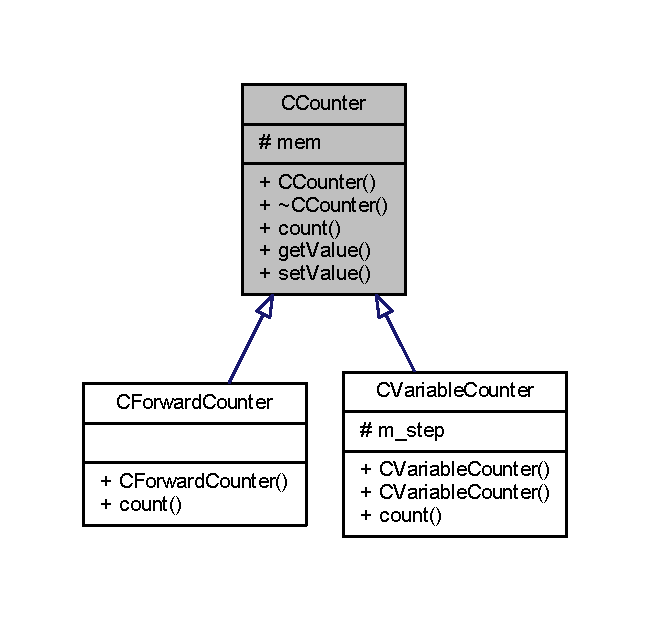
\includegraphics[width=312pt]{class_c_counter__inherit__graph}
\end{center}
\end{figure}


Zusammengehörigkeiten von C\+Counter\+:
\nopagebreak
\begin{figure}[H]
\begin{center}
\leavevmode
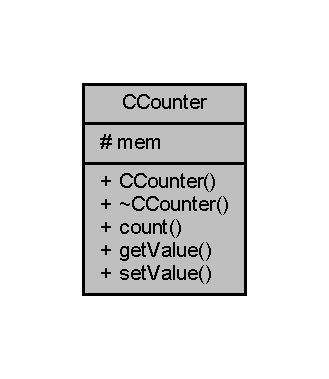
\includegraphics[width=158pt]{class_c_counter__coll__graph}
\end{center}
\end{figure}
\subsection*{Öffentliche Methoden}
\begin{DoxyCompactItemize}
\item 
\hyperlink{class_c_counter_ab83c6f9600beb5686747493da731a04c}{C\+Counter} ()
\item 
virtual \hyperlink{class_c_counter_a1af3cc000781fcd67b9e4fe1b25fbc9c}{$\sim$\+C\+Counter} ()
\item 
int \hyperlink{class_c_counter_ad91db4cd517159f7cbb7d3976eede482}{get\+Value} () const
\item 
void \hyperlink{class_c_counter_ac41245afdd95c0149e99bad21696a372}{set\+Value} (int value)
\item 
virtual void \hyperlink{class_c_counter_a90f3e164f3fc1dcf91044702d6940c4d}{count} ()
\item 
bool \hyperlink{class_c_counter_ac43e4c4cb447d22636ac208d426d95eb}{operator$<$} (const \hyperlink{class_c_counter}{C\+Counter} \&other) const
\item 
bool \hyperlink{class_c_counter_a23decf75e74ddfd25feb11ae6aad9c8a}{operator$>$} (const \hyperlink{class_c_counter}{C\+Counter} \&other) const
\end{DoxyCompactItemize}


\subsection{Ausführliche Beschreibung}
Klasse \hyperlink{class_c_counter}{C\+Counter} zum Setzen, Inkrementieren und Vergleichen von Zählerständen. 

\hyperlink{class_c_counter_ab83c6f9600beb5686747493da731a04c}{C\+Counter()} ist der parameterlose Konstruktor \hyperlink{class_c_counter_a1af3cc000781fcd67b9e4fe1b25fbc9c}{$\sim$\+C\+Counter()} ist der Destruktor int \hyperlink{class_c_counter_ad91db4cd517159f7cbb7d3976eede482}{get\+Value()} liefert den Zählerstand void \hyperlink{class_c_counter_ac41245afdd95c0149e99bad21696a372}{set\+Value(int)} setzt den Zählerstand void \hyperlink{class_c_counter_a90f3e164f3fc1dcf91044702d6940c4d}{count()} inkrementiert den Zählerstand bool operator$<$(\+C\+Counter\&) prüft, ob Argument größeren Zählerstand besitzt bool operator$>$(\+C\+Counter\&)

int m\+\_\+value ist die private Membervariable für den Zählerstand. Wir verwenden die Konvention, dass der Namen privater Membervariablen mit m\+\_\+ beginnt. 

\subsection{Beschreibung der Konstruktoren und Destruktoren}
\mbox{\Hypertarget{class_c_counter_ab83c6f9600beb5686747493da731a04c}\label{class_c_counter_ab83c6f9600beb5686747493da731a04c}} 
\index{C\+Counter@{C\+Counter}!C\+Counter@{C\+Counter}}
\index{C\+Counter@{C\+Counter}!C\+Counter@{C\+Counter}}
\subsubsection{\texorpdfstring{C\+Counter()}{CCounter()}}
{\footnotesize\ttfamily C\+Counter\+::\+C\+Counter (\begin{DoxyParamCaption}{ }\end{DoxyParamCaption})}

Deklaration des parameterlosen Konstruktors. \mbox{\Hypertarget{class_c_counter_a1af3cc000781fcd67b9e4fe1b25fbc9c}\label{class_c_counter_a1af3cc000781fcd67b9e4fe1b25fbc9c}} 
\index{C\+Counter@{C\+Counter}!````~C\+Counter@{$\sim$\+C\+Counter}}
\index{````~C\+Counter@{$\sim$\+C\+Counter}!C\+Counter@{C\+Counter}}
\subsubsection{\texorpdfstring{$\sim$\+C\+Counter()}{~CCounter()}}
{\footnotesize\ttfamily C\+Counter\+::$\sim$\+C\+Counter (\begin{DoxyParamCaption}{ }\end{DoxyParamCaption})\hspace{0.3cm}{\ttfamily [virtual]}}

Destruktor von \hyperlink{class_c_counter}{C\+Counter} 

\subsection{Dokumentation der Elementfunktionen}
\mbox{\Hypertarget{class_c_counter_a90f3e164f3fc1dcf91044702d6940c4d}\label{class_c_counter_a90f3e164f3fc1dcf91044702d6940c4d}} 
\index{C\+Counter@{C\+Counter}!count@{count}}
\index{count@{count}!C\+Counter@{C\+Counter}}
\subsubsection{\texorpdfstring{count()}{count()}}
{\footnotesize\ttfamily void C\+Counter\+::count (\begin{DoxyParamCaption}{ }\end{DoxyParamCaption})\hspace{0.3cm}{\ttfamily [virtual]}}

Inkrementiert den Zählerstand um 1 

Erneute Implementation in \hyperlink{class_c_variable_counter_a693c27202acd18d53c4642ce642927bc}{C\+Variable\+Counter} und \hyperlink{class_c_forward_counter_afc451afa9f8b76f70b28c08982265a86}{C\+Forward\+Counter}.

Hier ist ein Graph der zeigt, wo diese Funktion aufgerufen wird\+:
\nopagebreak
\begin{figure}[H]
\begin{center}
\leavevmode
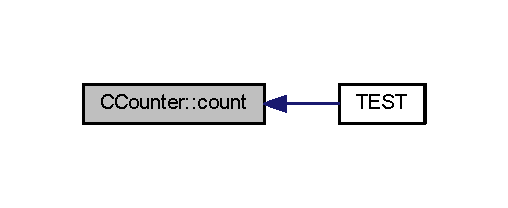
\includegraphics[width=244pt]{class_c_counter_a90f3e164f3fc1dcf91044702d6940c4d_icgraph}
\end{center}
\end{figure}
\mbox{\Hypertarget{class_c_counter_ad91db4cd517159f7cbb7d3976eede482}\label{class_c_counter_ad91db4cd517159f7cbb7d3976eede482}} 
\index{C\+Counter@{C\+Counter}!get\+Value@{get\+Value}}
\index{get\+Value@{get\+Value}!C\+Counter@{C\+Counter}}
\subsubsection{\texorpdfstring{get\+Value()}{getValue()}}
{\footnotesize\ttfamily int C\+Counter\+::get\+Value (\begin{DoxyParamCaption}{ }\end{DoxyParamCaption}) const}

Gib den Wert der Zählervariable aus. \begin{DoxyReturn}{Rückgabe}
enthält den Wert der Zählervariable m\+\_\+value. 
\end{DoxyReturn}
Hier ist ein Graph der zeigt, wo diese Funktion aufgerufen wird\+:
\nopagebreak
\begin{figure}[H]
\begin{center}
\leavevmode
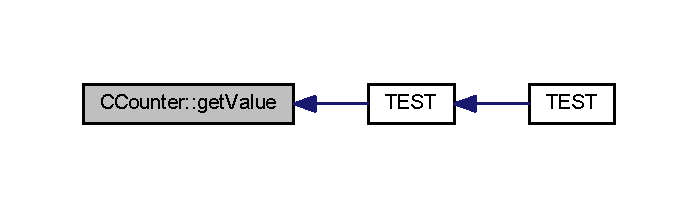
\includegraphics[width=335pt]{class_c_counter_ad91db4cd517159f7cbb7d3976eede482_icgraph}
\end{center}
\end{figure}
\mbox{\Hypertarget{class_c_counter_ac43e4c4cb447d22636ac208d426d95eb}\label{class_c_counter_ac43e4c4cb447d22636ac208d426d95eb}} 
\index{C\+Counter@{C\+Counter}!operator$<$@{operator$<$}}
\index{operator$<$@{operator$<$}!C\+Counter@{C\+Counter}}
\subsubsection{\texorpdfstring{operator$<$()}{operator<()}}
{\footnotesize\ttfamily bool C\+Counter\+::operator$<$ (\begin{DoxyParamCaption}\item[{const \hyperlink{class_c_counter}{C\+Counter} \&}]{other }\end{DoxyParamCaption}) const}

Prüft, ob der Zählerstand kleiner ist, als der Eingabeparameter. Die Memberfunktion \hyperlink{class_c_counter_ac43e4c4cb447d22636ac208d426d95eb}{operator$<$()} steht für den Operator $<$ . 
\begin{DoxyParams}{Parameter}
{\em other} & ist der Eingabeparameter. \\
\hline
\end{DoxyParams}
\begin{DoxyReturn}{Rückgabe}
ist wahr, falls der Zählerstand kleiner als der Eingabeparameter ist. 
\end{DoxyReturn}
\mbox{\Hypertarget{class_c_counter_a23decf75e74ddfd25feb11ae6aad9c8a}\label{class_c_counter_a23decf75e74ddfd25feb11ae6aad9c8a}} 
\index{C\+Counter@{C\+Counter}!operator$>$@{operator$>$}}
\index{operator$>$@{operator$>$}!C\+Counter@{C\+Counter}}
\subsubsection{\texorpdfstring{operator$>$()}{operator>()}}
{\footnotesize\ttfamily bool C\+Counter\+::operator$>$ (\begin{DoxyParamCaption}\item[{const \hyperlink{class_c_counter}{C\+Counter} \&}]{other }\end{DoxyParamCaption}) const}

Prüft, ob der Zählerstand größer ist, als der Eingabeparameter. Die Memberfunktion \hyperlink{class_c_counter_a23decf75e74ddfd25feb11ae6aad9c8a}{operator$>$()} steht für den Operator $>$ . 
\begin{DoxyParams}{Parameter}
{\em other} & ist der Eingabeparameter. \\
\hline
\end{DoxyParams}
\begin{DoxyReturn}{Rückgabe}
ist wahr, falls der Zählerstand größer als der Eingabeparameter ist. 
\end{DoxyReturn}
\mbox{\Hypertarget{class_c_counter_ac41245afdd95c0149e99bad21696a372}\label{class_c_counter_ac41245afdd95c0149e99bad21696a372}} 
\index{C\+Counter@{C\+Counter}!set\+Value@{set\+Value}}
\index{set\+Value@{set\+Value}!C\+Counter@{C\+Counter}}
\subsubsection{\texorpdfstring{set\+Value()}{setValue()}}
{\footnotesize\ttfamily void C\+Counter\+::set\+Value (\begin{DoxyParamCaption}\item[{int}]{value }\end{DoxyParamCaption})}

Setze die Zählervariable. 
\begin{DoxyParams}{Parameter}
{\em value} & Die Zählervariable m\+\_\+value wird auf den Wert der Parametervariable value gesetzt. \\
\hline
\end{DoxyParams}
Hier ist ein Graph der zeigt, wo diese Funktion aufgerufen wird\+:
\nopagebreak
\begin{figure}[H]
\begin{center}
\leavevmode
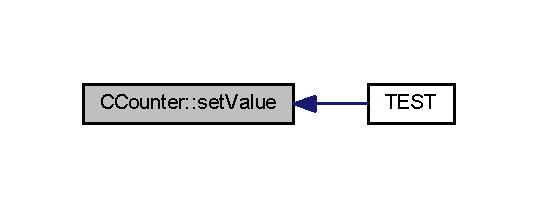
\includegraphics[width=258pt]{class_c_counter_ac41245afdd95c0149e99bad21696a372_icgraph}
\end{center}
\end{figure}


Die Dokumentation für diese Klasse wurde erzeugt aufgrund der Dateien\+:\begin{DoxyCompactItemize}
\item 
C\+:/portable\+Dev\+Env\+\_\+2017/workspace2017/\+Blatt2/src/\hyperlink{_c_counter_8hpp}{C\+Counter.\+hpp}\item 
C\+:/portable\+Dev\+Env\+\_\+2017/workspace2017/\+Blatt2/src/\hyperlink{_c_counter_8cpp}{C\+Counter.\+cpp}\end{DoxyCompactItemize}

\hypertarget{class_c_forward_counter}{}\section{C\+Forward\+Counter Klassenreferenz}
\label{class_c_forward_counter}\index{C\+Forward\+Counter@{C\+Forward\+Counter}}


{\ttfamily \#include $<$C\+Forward\+Counter.\+hpp$>$}



Klassendiagramm für C\+Forward\+Counter\+:
\nopagebreak
\begin{figure}[H]
\begin{center}
\leavevmode
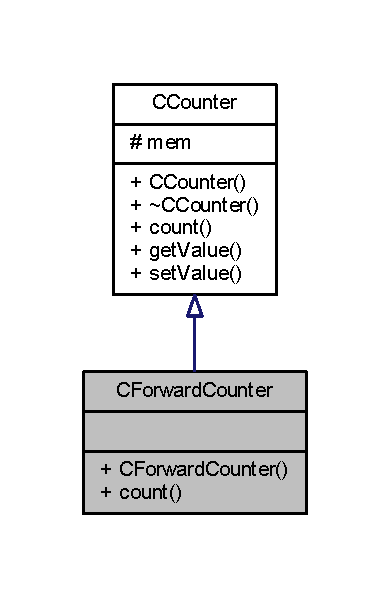
\includegraphics[width=187pt]{class_c_forward_counter__inherit__graph}
\end{center}
\end{figure}


Zusammengehörigkeiten von C\+Forward\+Counter\+:
\nopagebreak
\begin{figure}[H]
\begin{center}
\leavevmode
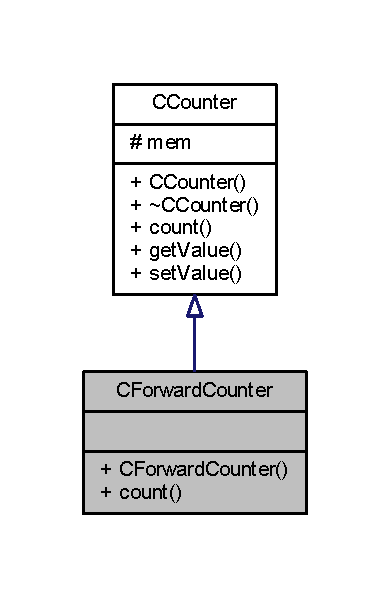
\includegraphics[width=187pt]{class_c_forward_counter__coll__graph}
\end{center}
\end{figure}
\subsection*{Öffentliche Methoden}
\begin{DoxyCompactItemize}
\item 
\hyperlink{class_c_forward_counter_aeda1b05d715820f61e377a2c6fa52b2e}{C\+Forward\+Counter} ()
\item 
void \hyperlink{class_c_forward_counter_afc451afa9f8b76f70b28c08982265a86}{count} ()
\end{DoxyCompactItemize}


\subsection{Ausführliche Beschreibung}
\hyperlink{class_c_forward_counter}{C\+Forward\+Counter}, überschreibt die Memberfunktion \hyperlink{class_c_forward_counter_afc451afa9f8b76f70b28c08982265a86}{count()} aus Basisklasse \hyperlink{class_c_counter}{C\+Counter}, so dass diese den internen Zählerstand um 1 inkrementiert. 

\subsection{Beschreibung der Konstruktoren und Destruktoren}
\mbox{\Hypertarget{class_c_forward_counter_aeda1b05d715820f61e377a2c6fa52b2e}\label{class_c_forward_counter_aeda1b05d715820f61e377a2c6fa52b2e}} 
\index{C\+Forward\+Counter@{C\+Forward\+Counter}!C\+Forward\+Counter@{C\+Forward\+Counter}}
\index{C\+Forward\+Counter@{C\+Forward\+Counter}!C\+Forward\+Counter@{C\+Forward\+Counter}}
\subsubsection{\texorpdfstring{C\+Forward\+Counter()}{CForwardCounter()}}
{\footnotesize\ttfamily C\+Forward\+Counter\+::\+C\+Forward\+Counter (\begin{DoxyParamCaption}{ }\end{DoxyParamCaption})}

Parameterloser Konstruktor, setzt den Zählerstand auf 0 

\subsection{Dokumentation der Elementfunktionen}
\mbox{\Hypertarget{class_c_forward_counter_afc451afa9f8b76f70b28c08982265a86}\label{class_c_forward_counter_afc451afa9f8b76f70b28c08982265a86}} 
\index{C\+Forward\+Counter@{C\+Forward\+Counter}!count@{count}}
\index{count@{count}!C\+Forward\+Counter@{C\+Forward\+Counter}}
\subsubsection{\texorpdfstring{count()}{count()}}
{\footnotesize\ttfamily void C\+Forward\+Counter\+::count (\begin{DoxyParamCaption}{ }\end{DoxyParamCaption})\hspace{0.3cm}{\ttfamily [virtual]}}

Zähler, inkrementiert den Zählerstand um 1 

Erneute Implementation von \hyperlink{class_c_counter_a90f3e164f3fc1dcf91044702d6940c4d}{C\+Counter}.

Hier ist ein Graph der zeigt, wo diese Funktion aufgerufen wird\+:
\nopagebreak
\begin{figure}[H]
\begin{center}
\leavevmode
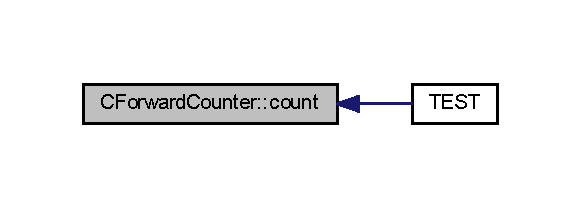
\includegraphics[width=279pt]{class_c_forward_counter_afc451afa9f8b76f70b28c08982265a86_icgraph}
\end{center}
\end{figure}


Die Dokumentation für diese Klasse wurde erzeugt aufgrund der Dateien\+:\begin{DoxyCompactItemize}
\item 
C\+:/portable\+Dev\+Env\+\_\+2017/workspace2017/\+Blatt2/src/\hyperlink{_c_forward_counter_8hpp}{C\+Forward\+Counter.\+hpp}\item 
C\+:/portable\+Dev\+Env\+\_\+2017/workspace2017/\+Blatt2/src/\hyperlink{_c_forward_counter_8cpp}{C\+Forward\+Counter.\+cpp}\end{DoxyCompactItemize}

\hypertarget{class_c_variable_counter}{}\section{C\+Variable\+Counter Klassenreferenz}
\label{class_c_variable_counter}\index{C\+Variable\+Counter@{C\+Variable\+Counter}}


{\ttfamily \#include $<$C\+Variable\+Counter.\+hpp$>$}



Klassendiagramm für C\+Variable\+Counter\+:
\nopagebreak
\begin{figure}[H]
\begin{center}
\leavevmode
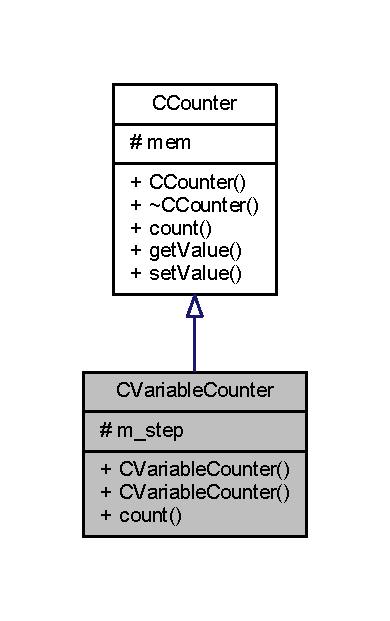
\includegraphics[width=187pt]{class_c_variable_counter__inherit__graph}
\end{center}
\end{figure}


Zusammengehörigkeiten von C\+Variable\+Counter\+:
\nopagebreak
\begin{figure}[H]
\begin{center}
\leavevmode
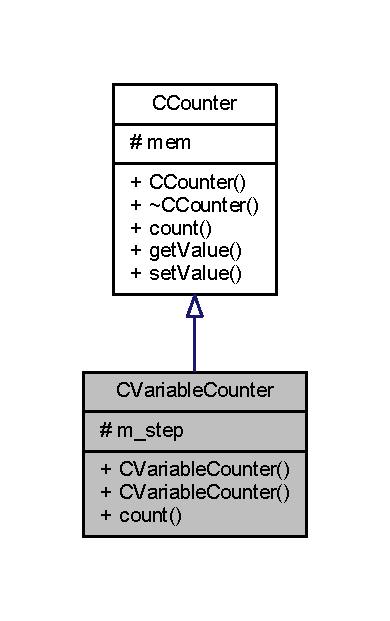
\includegraphics[width=187pt]{class_c_variable_counter__coll__graph}
\end{center}
\end{figure}
\subsection*{Öffentliche Methoden}
\begin{DoxyCompactItemize}
\item 
\hyperlink{class_c_variable_counter_a76f4aa9bc231429b02678050eec85518}{C\+Variable\+Counter} ()
\item 
\hyperlink{class_c_variable_counter_a80ffababfaed8740dcccc1958416dc81}{C\+Variable\+Counter} (int step)
\item 
void \hyperlink{class_c_variable_counter_a693c27202acd18d53c4642ce642927bc}{count} ()
\end{DoxyCompactItemize}
\subsection*{Geschützte Attribute}
\begin{DoxyCompactItemize}
\item 
int \hyperlink{class_c_variable_counter_a970fd88636f33c50c7c3005f92bebf87}{m\+\_\+step}
\begin{DoxyCompactList}\small\item\em Schrittvariable. \end{DoxyCompactList}\end{DoxyCompactItemize}


\subsection{Beschreibung der Konstruktoren und Destruktoren}
\mbox{\Hypertarget{class_c_variable_counter_a76f4aa9bc231429b02678050eec85518}\label{class_c_variable_counter_a76f4aa9bc231429b02678050eec85518}} 
\index{C\+Variable\+Counter@{C\+Variable\+Counter}!C\+Variable\+Counter@{C\+Variable\+Counter}}
\index{C\+Variable\+Counter@{C\+Variable\+Counter}!C\+Variable\+Counter@{C\+Variable\+Counter}}
\subsubsection{\texorpdfstring{C\+Variable\+Counter()}{CVariableCounter()}\hspace{0.1cm}{\footnotesize\ttfamily [1/2]}}
{\footnotesize\ttfamily C\+Variable\+Counter\+::\+C\+Variable\+Counter (\begin{DoxyParamCaption}{ }\end{DoxyParamCaption})}

Konstruktor, m\+\_\+step normal mit 0 initialisiert \mbox{\Hypertarget{class_c_variable_counter_a80ffababfaed8740dcccc1958416dc81}\label{class_c_variable_counter_a80ffababfaed8740dcccc1958416dc81}} 
\index{C\+Variable\+Counter@{C\+Variable\+Counter}!C\+Variable\+Counter@{C\+Variable\+Counter}}
\index{C\+Variable\+Counter@{C\+Variable\+Counter}!C\+Variable\+Counter@{C\+Variable\+Counter}}
\subsubsection{\texorpdfstring{C\+Variable\+Counter()}{CVariableCounter()}\hspace{0.1cm}{\footnotesize\ttfamily [2/2]}}
{\footnotesize\ttfamily C\+Variable\+Counter\+::\+C\+Variable\+Counter (\begin{DoxyParamCaption}\item[{int}]{step }\end{DoxyParamCaption})}

Konstruktor 
\begin{DoxyParams}{Parameter}
{\em step} & Schrittgröße \\
\hline
\end{DoxyParams}


\subsection{Dokumentation der Elementfunktionen}
\mbox{\Hypertarget{class_c_variable_counter_a693c27202acd18d53c4642ce642927bc}\label{class_c_variable_counter_a693c27202acd18d53c4642ce642927bc}} 
\index{C\+Variable\+Counter@{C\+Variable\+Counter}!count@{count}}
\index{count@{count}!C\+Variable\+Counter@{C\+Variable\+Counter}}
\subsubsection{\texorpdfstring{count()}{count()}}
{\footnotesize\ttfamily void C\+Variable\+Counter\+::count (\begin{DoxyParamCaption}{ }\end{DoxyParamCaption})\hspace{0.3cm}{\ttfamily [virtual]}}

Zählfunktion 

Erneute Implementation von \hyperlink{class_c_counter_a90f3e164f3fc1dcf91044702d6940c4d}{C\+Counter}.

Hier ist ein Graph der zeigt, wo diese Funktion aufgerufen wird\+:\nopagebreak
\begin{figure}[H]
\begin{center}
\leavevmode
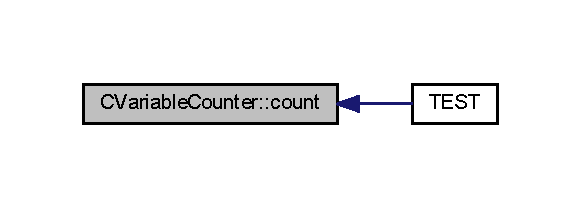
\includegraphics[width=279pt]{class_c_variable_counter_a693c27202acd18d53c4642ce642927bc_icgraph}
\end{center}
\end{figure}


\subsection{Dokumentation der Datenelemente}
\mbox{\Hypertarget{class_c_variable_counter_a970fd88636f33c50c7c3005f92bebf87}\label{class_c_variable_counter_a970fd88636f33c50c7c3005f92bebf87}} 
\index{C\+Variable\+Counter@{C\+Variable\+Counter}!m\+\_\+step@{m\+\_\+step}}
\index{m\+\_\+step@{m\+\_\+step}!C\+Variable\+Counter@{C\+Variable\+Counter}}
\subsubsection{\texorpdfstring{m\+\_\+step}{m\_step}}
{\footnotesize\ttfamily int C\+Variable\+Counter\+::m\+\_\+step\hspace{0.3cm}{\ttfamily [protected]}}



Schrittvariable. 



Die Dokumentation für diese Klasse wurde erzeugt aufgrund der Dateien\+:\begin{DoxyCompactItemize}
\item 
C\+:/portable\+Dev\+Env\+\_\+2017/workspace2017/\+S\+\_\+\+Blatt2/src/\hyperlink{_c_variable_counter_8hpp}{C\+Variable\+Counter.\+hpp}\item 
C\+:/portable\+Dev\+Env\+\_\+2017/workspace2017/\+S\+\_\+\+Blatt2/src/\hyperlink{_c_variable_counter_8cpp}{C\+Variable\+Counter.\+cpp}\end{DoxyCompactItemize}

\chapter{Datei-\/\+Dokumentation}
\hypertarget{ccounter_8cpp}{}\section{C\+:/portable\+Dev\+Env\+\_\+2017/workspace2017/\+S\+\_\+\+Blatt2/src/ccounter.cpp-\/\+Dateireferenz}
\label{ccounter_8cpp}\index{C\+:/portable\+Dev\+Env\+\_\+2017/workspace2017/\+S\+\_\+\+Blatt2/src/ccounter.\+cpp@{C\+:/portable\+Dev\+Env\+\_\+2017/workspace2017/\+S\+\_\+\+Blatt2/src/ccounter.\+cpp}}


Created on\+: 06.\+04.\+2018 Author\+: diamo.  


{\ttfamily \#include \char`\"{}ccounter.\+hpp\char`\"{}}\newline
Include-\/\+Abhängigkeitsdiagramm für ccounter.\+cpp\+:\nopagebreak
\begin{figure}[H]
\begin{center}
\leavevmode
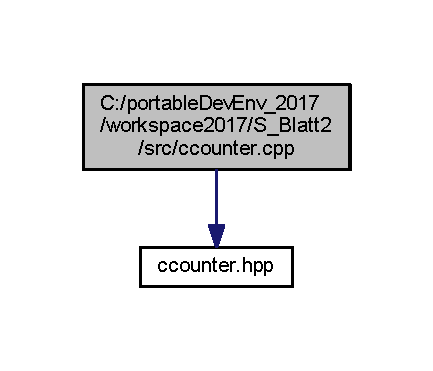
\includegraphics[width=208pt]{ccounter_8cpp__incl}
\end{center}
\end{figure}


\subsection{Ausführliche Beschreibung}
Created on\+: 06.\+04.\+2018 Author\+: diamo. 


\hypertarget{ccounter_8hpp}{}\section{C\+:/portable\+Dev\+Env\+\_\+2017/workspace2017/\+S\+\_\+\+Blatt2/src/ccounter.hpp-\/\+Dateireferenz}
\label{ccounter_8hpp}\index{C\+:/portable\+Dev\+Env\+\_\+2017/workspace2017/\+S\+\_\+\+Blatt2/src/ccounter.\+hpp@{C\+:/portable\+Dev\+Env\+\_\+2017/workspace2017/\+S\+\_\+\+Blatt2/src/ccounter.\+hpp}}


Created on\+: 06.\+04.\+2018 Author\+: diamo.  


Dieser Graph zeigt, welche Datei direkt oder indirekt diese Datei enthält\+:\nopagebreak
\begin{figure}[H]
\begin{center}
\leavevmode
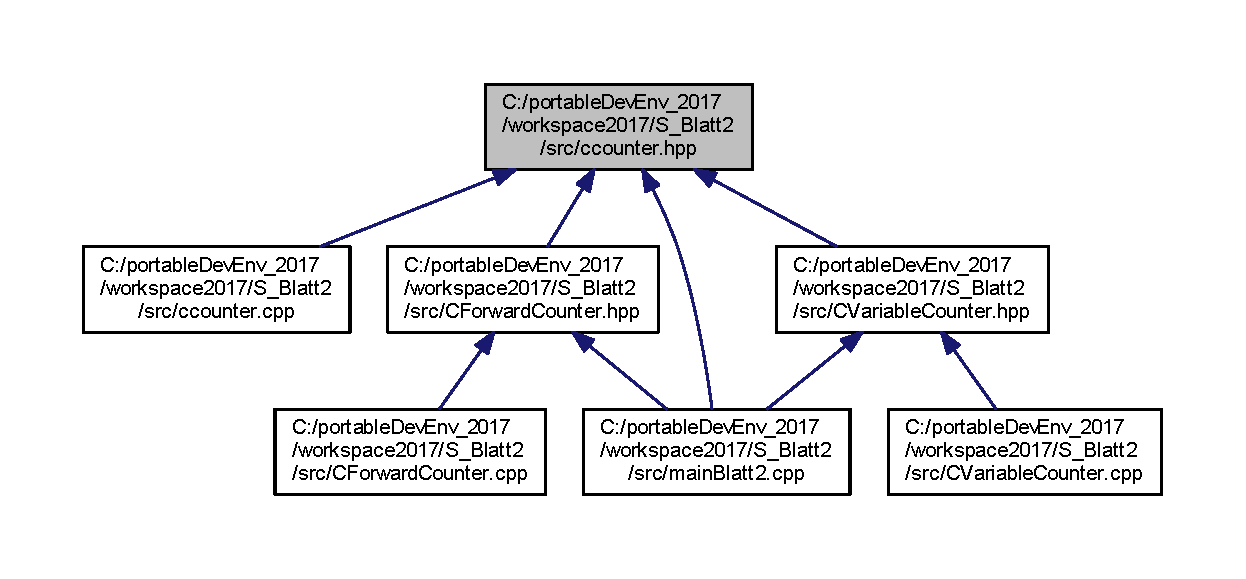
\includegraphics[width=350pt]{ccounter_8hpp__dep__incl}
\end{center}
\end{figure}
\subsection*{Klassen}
\begin{DoxyCompactItemize}
\item 
class \hyperlink{class_c_counter}{C\+Counter}
\end{DoxyCompactItemize}


\subsection{Ausführliche Beschreibung}
Created on\+: 06.\+04.\+2018 Author\+: diamo. 


\hypertarget{_c_forward_counter_8cpp}{}\section{C\+:/portable\+Dev\+Env\+\_\+2017/workspace2017/\+S\+\_\+\+Blatt2/src/\+C\+Forward\+Counter.cpp-\/\+Dateireferenz}
\label{_c_forward_counter_8cpp}\index{C\+:/portable\+Dev\+Env\+\_\+2017/workspace2017/\+S\+\_\+\+Blatt2/src/\+C\+Forward\+Counter.\+cpp@{C\+:/portable\+Dev\+Env\+\_\+2017/workspace2017/\+S\+\_\+\+Blatt2/src/\+C\+Forward\+Counter.\+cpp}}


Created on\+: 07.\+04.\+2018 Author\+: diamo.  


{\ttfamily \#include \char`\"{}C\+Forward\+Counter.\+hpp\char`\"{}}\newline
Include-\/\+Abhängigkeitsdiagramm für C\+Forward\+Counter.\+cpp\+:\nopagebreak
\begin{figure}[H]
\begin{center}
\leavevmode
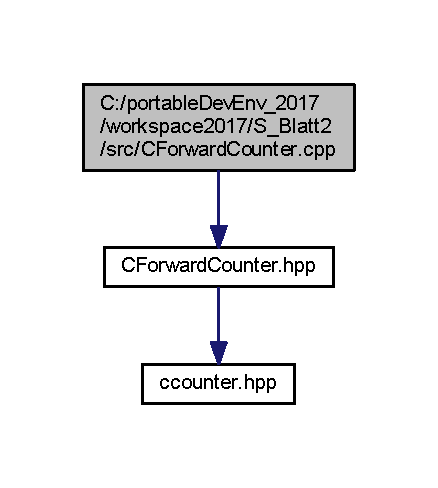
\includegraphics[width=210pt]{_c_forward_counter_8cpp__incl}
\end{center}
\end{figure}


\subsection{Ausführliche Beschreibung}
Created on\+: 07.\+04.\+2018 Author\+: diamo. 


\hypertarget{_c_forward_counter_8hpp}{}\section{C\+:/portable\+Dev\+Env\+\_\+2017/workspace2017/project/src/\+C\+Forward\+Counter.hpp-\/\+Dateireferenz}
\label{_c_forward_counter_8hpp}\index{C\+:/portable\+Dev\+Env\+\_\+2017/workspace2017/project/src/\+C\+Forward\+Counter.\+hpp@{C\+:/portable\+Dev\+Env\+\_\+2017/workspace2017/project/src/\+C\+Forward\+Counter.\+hpp}}


Created on\+: 07.\+04.\+2018 Author\+: diamo.  


{\ttfamily \#include \char`\"{}C\+Counter.\+hpp\char`\"{}}\newline
Include-\/\+Abhängigkeitsdiagramm für C\+Forward\+Counter.\+hpp\+:
\nopagebreak
\begin{figure}[H]
\begin{center}
\leavevmode
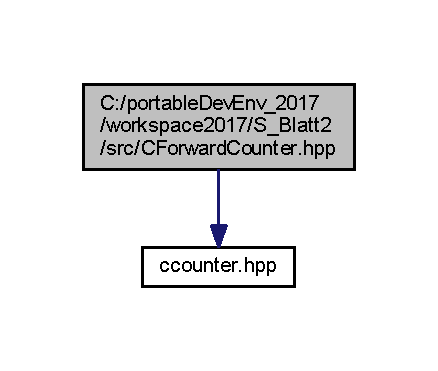
\includegraphics[width=210pt]{_c_forward_counter_8hpp__incl}
\end{center}
\end{figure}
Dieser Graph zeigt, welche Datei direkt oder indirekt diese Datei enthält\+:
\nopagebreak
\begin{figure}[H]
\begin{center}
\leavevmode
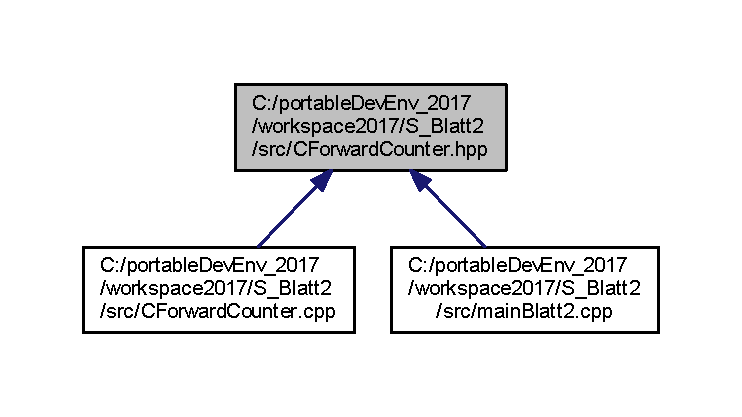
\includegraphics[width=350pt]{_c_forward_counter_8hpp__dep__incl}
\end{center}
\end{figure}
\subsection*{Klassen}
\begin{DoxyCompactItemize}
\item 
class \hyperlink{class_c_forward_counter}{C\+Forward\+Counter}
\end{DoxyCompactItemize}


\subsection{Ausführliche Beschreibung}
Created on\+: 07.\+04.\+2018 Author\+: diamo. 


\hypertarget{_c_variable_counter_8cpp}{}\section{C\+:/portable\+Dev\+Env\+\_\+2017/workspace2017/\+S\+\_\+\+Blatt2/src/\+C\+Variable\+Counter.cpp-\/\+Dateireferenz}
\label{_c_variable_counter_8cpp}\index{C\+:/portable\+Dev\+Env\+\_\+2017/workspace2017/\+S\+\_\+\+Blatt2/src/\+C\+Variable\+Counter.\+cpp@{C\+:/portable\+Dev\+Env\+\_\+2017/workspace2017/\+S\+\_\+\+Blatt2/src/\+C\+Variable\+Counter.\+cpp}}


Created on\+: 07.\+04.\+2018 Author\+: diamo.  


{\ttfamily \#include \char`\"{}C\+Variable\+Counter.\+hpp\char`\"{}}\newline
Include-\/\+Abhängigkeitsdiagramm für C\+Variable\+Counter.\+cpp\+:\nopagebreak
\begin{figure}[H]
\begin{center}
\leavevmode
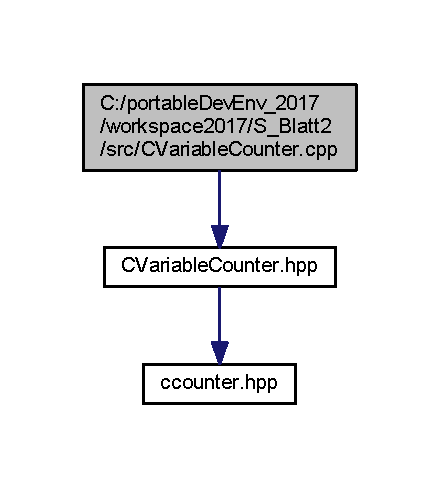
\includegraphics[width=211pt]{_c_variable_counter_8cpp__incl}
\end{center}
\end{figure}


\subsection{Ausführliche Beschreibung}
Created on\+: 07.\+04.\+2018 Author\+: diamo. 


\hypertarget{_c_variable_counter_8hpp}{}\section{C\+:/portable\+Dev\+Env\+\_\+2017/workspace2017/\+S\+\_\+\+Blatt2/src/\+C\+Variable\+Counter.hpp-\/\+Dateireferenz}
\label{_c_variable_counter_8hpp}\index{C\+:/portable\+Dev\+Env\+\_\+2017/workspace2017/\+S\+\_\+\+Blatt2/src/\+C\+Variable\+Counter.\+hpp@{C\+:/portable\+Dev\+Env\+\_\+2017/workspace2017/\+S\+\_\+\+Blatt2/src/\+C\+Variable\+Counter.\+hpp}}


Created on\+: 07.\+04.\+2018 Author\+: diamo.  


{\ttfamily \#include \char`\"{}ccounter.\+hpp\char`\"{}}\newline
Include-\/\+Abhängigkeitsdiagramm für C\+Variable\+Counter.\+hpp\+:\nopagebreak
\begin{figure}[H]
\begin{center}
\leavevmode
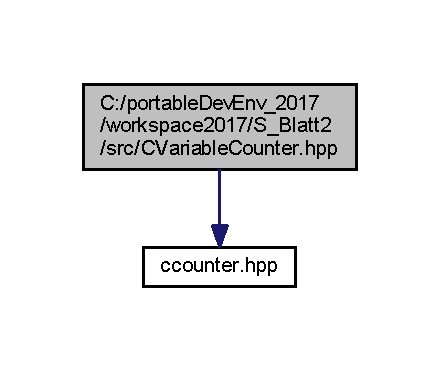
\includegraphics[width=211pt]{_c_variable_counter_8hpp__incl}
\end{center}
\end{figure}
Dieser Graph zeigt, welche Datei direkt oder indirekt diese Datei enthält\+:\nopagebreak
\begin{figure}[H]
\begin{center}
\leavevmode
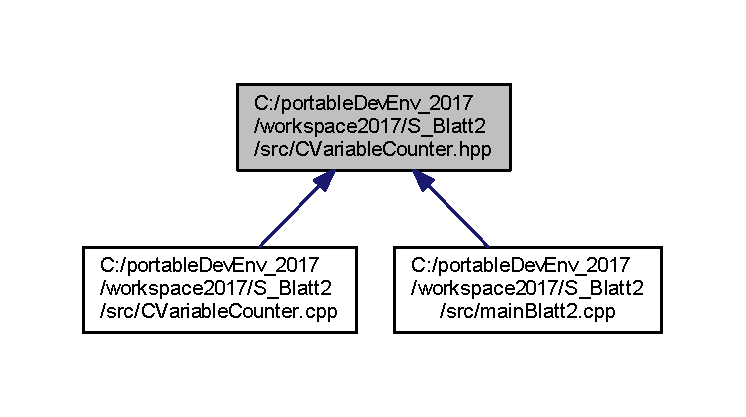
\includegraphics[width=350pt]{_c_variable_counter_8hpp__dep__incl}
\end{center}
\end{figure}
\subsection*{Klassen}
\begin{DoxyCompactItemize}
\item 
class \hyperlink{class_c_variable_counter}{C\+Variable\+Counter}
\end{DoxyCompactItemize}


\subsection{Ausführliche Beschreibung}
Created on\+: 07.\+04.\+2018 Author\+: diamo. 


\hypertarget{main_blatt2_8cpp}{}\section{C\+:/portable\+Dev\+Env\+\_\+2017/workspace2017/\+Blatt2/src/main\+Blatt2.cpp-\/\+Dateireferenz}
\label{main_blatt2_8cpp}\index{C\+:/portable\+Dev\+Env\+\_\+2017/workspace2017/\+Blatt2/src/main\+Blatt2.\+cpp@{C\+:/portable\+Dev\+Env\+\_\+2017/workspace2017/\+Blatt2/src/main\+Blatt2.\+cpp}}
{\ttfamily \#include $<$iostream$>$}\newline
{\ttfamily \#include \char`\"{}gtest/gtest.\+h\char`\"{}}\newline
{\ttfamily \#include \char`\"{}C\+Counter.\+hpp\char`\"{}}\newline
Include-\/\+Abhängigkeitsdiagramm für main\+Blatt2.\+cpp\+:
\nopagebreak
\begin{figure}[H]
\begin{center}
\leavevmode
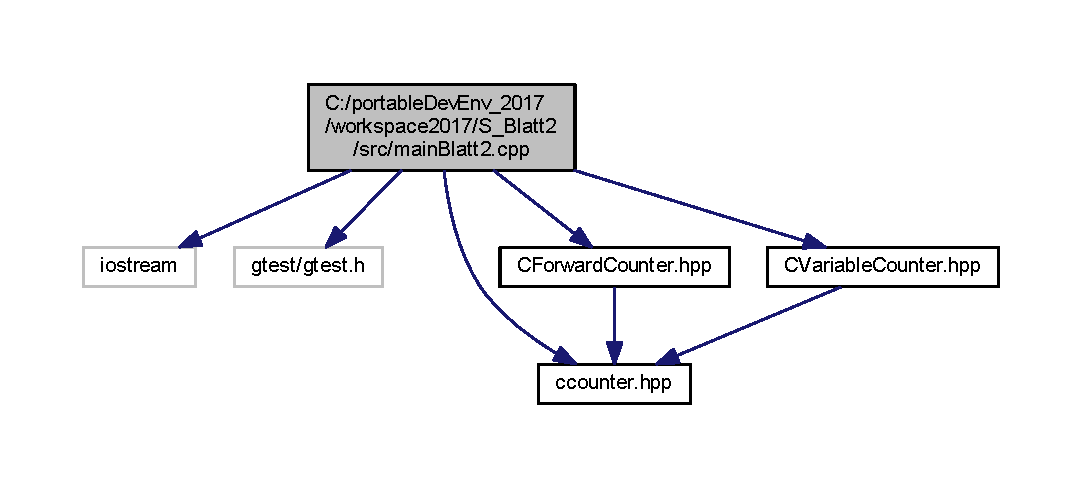
\includegraphics[width=318pt]{main_blatt2_8cpp__incl}
\end{center}
\end{figure}
\subsection*{Makrodefinitionen}
\begin{DoxyCompactItemize}
\item 
\#define \hyperlink{main_blatt2_8cpp_aee51f479e63646729bb45a2671a52f9c}{A\+U\+F\+G\+A\+B\+E\+\_\+2}
\end{DoxyCompactItemize}
\subsection*{Funktionen}
\begin{DoxyCompactItemize}
\item 
\hyperlink{main_blatt2_8cpp_ac1913089df62097c77c6095ae8a8c29b}{T\+E\+ST} (C\+Counter\+Test, Initial\+Zero)
\item 
\hyperlink{main_blatt2_8cpp_a6211b8808649d2390334057d567c6176}{T\+E\+ST} (C\+Counter\+Test, Set\+Value)
\item 
\hyperlink{main_blatt2_8cpp_a42ba5ff13dbd1ebf796bd21321b56f8e}{T\+E\+ST} (C\+Counter\+Test, Counting)
\item 
int \hyperlink{main_blatt2_8cpp_a3c04138a5bfe5d72780bb7e82a18e627}{main} (int argc, char $\ast$$\ast$argv)
\end{DoxyCompactItemize}


\subsection{Makro-\/\+Dokumentation}
\mbox{\Hypertarget{main_blatt2_8cpp_aee51f479e63646729bb45a2671a52f9c}\label{main_blatt2_8cpp_aee51f479e63646729bb45a2671a52f9c}} 
\index{main\+Blatt2.\+cpp@{main\+Blatt2.\+cpp}!A\+U\+F\+G\+A\+B\+E\+\_\+2@{A\+U\+F\+G\+A\+B\+E\+\_\+2}}
\index{A\+U\+F\+G\+A\+B\+E\+\_\+2@{A\+U\+F\+G\+A\+B\+E\+\_\+2}!main\+Blatt2.\+cpp@{main\+Blatt2.\+cpp}}
\subsubsection{\texorpdfstring{A\+U\+F\+G\+A\+B\+E\+\_\+2}{AUFGABE\_2}}
{\footnotesize\ttfamily \#define A\+U\+F\+G\+A\+B\+E\+\_\+2}



\subsection{Dokumentation der Funktionen}
\mbox{\Hypertarget{main_blatt2_8cpp_a3c04138a5bfe5d72780bb7e82a18e627}\label{main_blatt2_8cpp_a3c04138a5bfe5d72780bb7e82a18e627}} 
\index{main\+Blatt2.\+cpp@{main\+Blatt2.\+cpp}!main@{main}}
\index{main@{main}!main\+Blatt2.\+cpp@{main\+Blatt2.\+cpp}}
\subsubsection{\texorpdfstring{main()}{main()}}
{\footnotesize\ttfamily int main (\begin{DoxyParamCaption}\item[{int}]{argc,  }\item[{char $\ast$$\ast$}]{argv }\end{DoxyParamCaption})}

Hauptprogramm \hyperlink{main_blatt2_8cpp_a3c04138a5bfe5d72780bb7e82a18e627}{main()} mit Google Test (einkommentieren für den Google Test)

Dieses Hauptprogramm führt den Google Test aus. 
\begin{DoxyParams}{Parameter}
{\em argc} & ist die Anzahl der Kommandozeilenparameter \\
\hline
{\em argv} & ist ein Array aus Zeigern auf Kommandozeilenparameter \\
\hline
\end{DoxyParams}
\begin{DoxyReturn}{Rückgabe}
liefert 0, wenn alle Google Tests fehlerfrei durchlaufen 
\end{DoxyReturn}
\mbox{\Hypertarget{main_blatt2_8cpp_ac1913089df62097c77c6095ae8a8c29b}\label{main_blatt2_8cpp_ac1913089df62097c77c6095ae8a8c29b}} 
\index{main\+Blatt2.\+cpp@{main\+Blatt2.\+cpp}!T\+E\+ST@{T\+E\+ST}}
\index{T\+E\+ST@{T\+E\+ST}!main\+Blatt2.\+cpp@{main\+Blatt2.\+cpp}}
\subsubsection{\texorpdfstring{T\+E\+S\+T()}{TEST()}\hspace{0.1cm}{\footnotesize\ttfamily [1/3]}}
{\footnotesize\ttfamily T\+E\+ST (\begin{DoxyParamCaption}\item[{C\+Counter\+Test}]{,  }\item[{Initial\+Zero}]{ }\end{DoxyParamCaption})}

Hier ist ein Graph, der zeigt, was diese Funktion aufruft\+:
\nopagebreak
\begin{figure}[H]
\begin{center}
\leavevmode
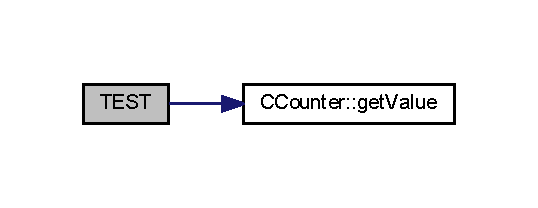
\includegraphics[width=258pt]{main_blatt2_8cpp_ac1913089df62097c77c6095ae8a8c29b_cgraph}
\end{center}
\end{figure}
Hier ist ein Graph der zeigt, wo diese Funktion aufgerufen wird\+:
\nopagebreak
\begin{figure}[H]
\begin{center}
\leavevmode
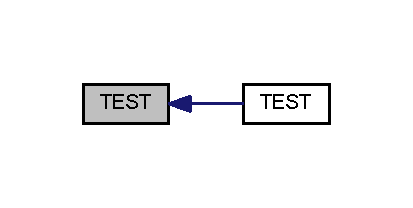
\includegraphics[width=198pt]{main_blatt2_8cpp_ac1913089df62097c77c6095ae8a8c29b_icgraph}
\end{center}
\end{figure}
\mbox{\Hypertarget{main_blatt2_8cpp_a6211b8808649d2390334057d567c6176}\label{main_blatt2_8cpp_a6211b8808649d2390334057d567c6176}} 
\index{main\+Blatt2.\+cpp@{main\+Blatt2.\+cpp}!T\+E\+ST@{T\+E\+ST}}
\index{T\+E\+ST@{T\+E\+ST}!main\+Blatt2.\+cpp@{main\+Blatt2.\+cpp}}
\subsubsection{\texorpdfstring{T\+E\+S\+T()}{TEST()}\hspace{0.1cm}{\footnotesize\ttfamily [2/3]}}
{\footnotesize\ttfamily T\+E\+ST (\begin{DoxyParamCaption}\item[{C\+Counter\+Test}]{,  }\item[{Set\+Value}]{ }\end{DoxyParamCaption})}

Hier ist ein Graph, der zeigt, was diese Funktion aufruft\+:
\nopagebreak
\begin{figure}[H]
\begin{center}
\leavevmode
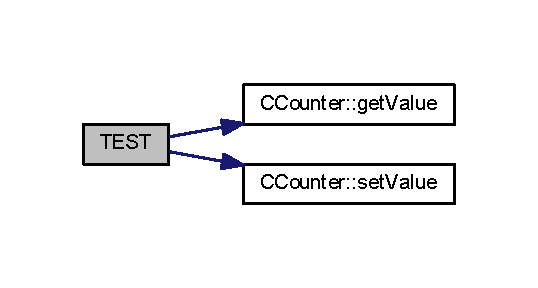
\includegraphics[width=258pt]{main_blatt2_8cpp_a6211b8808649d2390334057d567c6176_cgraph}
\end{center}
\end{figure}
\mbox{\Hypertarget{main_blatt2_8cpp_a42ba5ff13dbd1ebf796bd21321b56f8e}\label{main_blatt2_8cpp_a42ba5ff13dbd1ebf796bd21321b56f8e}} 
\index{main\+Blatt2.\+cpp@{main\+Blatt2.\+cpp}!T\+E\+ST@{T\+E\+ST}}
\index{T\+E\+ST@{T\+E\+ST}!main\+Blatt2.\+cpp@{main\+Blatt2.\+cpp}}
\subsubsection{\texorpdfstring{T\+E\+S\+T()}{TEST()}\hspace{0.1cm}{\footnotesize\ttfamily [3/3]}}
{\footnotesize\ttfamily T\+E\+ST (\begin{DoxyParamCaption}\item[{C\+Counter\+Test}]{,  }\item[{Counting}]{ }\end{DoxyParamCaption})}

Hier ist ein Graph, der zeigt, was diese Funktion aufruft\+:
\nopagebreak
\begin{figure}[H]
\begin{center}
\leavevmode
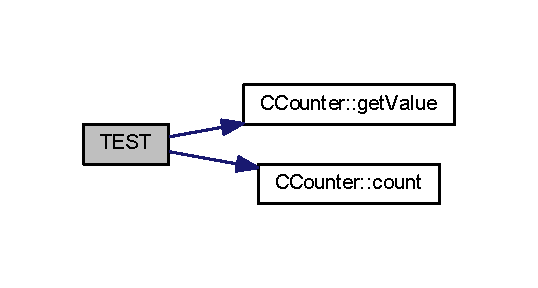
\includegraphics[width=350pt]{main_blatt2_8cpp_a42ba5ff13dbd1ebf796bd21321b56f8e_cgraph}
\end{center}
\end{figure}

%--- End generated contents ---

% Index
\backmatter
\newpage
\phantomsection
\clearemptydoublepage
\addcontentsline{toc}{chapter}{Index}
\printindex

\end{document}
